% Recommended preamble:
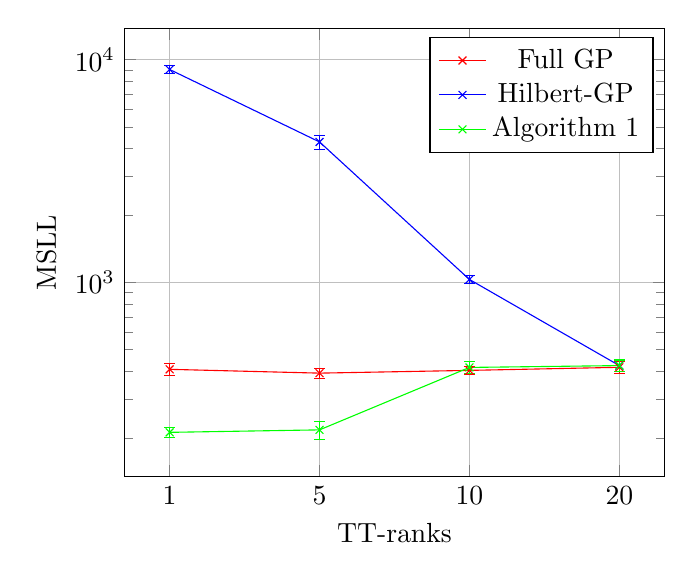
\begin{tikzpicture}
\begin{axis}[xmajorgrids, ymajorgrids, xlabel={TT-ranks}, ylabel={MSLL}, xtick={1,2,3,4}, xticklabels={1,5,10,20}, ymode={log}]
    \addplot[color={red}, mark={x}, error bars/y dir=both, error bars/y explicit]
        coordinates {
            (1,407.0679999999999) +- (0,25.256522717464055)
            (2,391.41459999999995) +- (0,19.50939565781917)
            (3,402.6471) +- (0,16.362111629887178)
            (4,415.6698) +- (0,24.453815293323856)
        }
        ;
    \addplot[color={blue}, mark={x}, error bars/y dir=both, error bars/y explicit]
        coordinates {
            (1,9043.961) +- (0,373.0179850132338)
            (2,4274.5419999999995) +- (0,305.6996731288915)
            (3,1031.0288) +- (0,39.81296914546536)
            (4,423.0996) +- (0,25.097492398865487)
        }
        ;
    \addplot[color={green}, mark={x}, error bars/y dir=both, error bars/y explicit]
        coordinates {
            (1,212.14569999999998) +- (0,11.186035848821119)
            (2,217.6529) +- (0,19.937475909842636)
            (3,415.16769999999997) +- (0,25.124882664402634)
            (4,423.0996) +- (0,25.097492398865487)
        }
        ;
    \legend{{Full GP},{Hilbert-GP},{Algorithm 1}}
\end{axis}
\end{tikzpicture}
